\newpage

\begin{center}
{\bf\LARGE 45neV parxkaraNa.}\\
\vskip .2cm
{\rm DIVISION OF DECIMALS.}
\vskip .2cm
{\bf\large dashAMsha apUNARMkiya BAgAkAravu.}
\vskip .2cm
{\bf\large sUtarx.}
\end{center}

\begin{verse}
kaM|| BAgisu Bajakadi BAjayxva| nAgalu pUNARMkiyaMte sheVSada muMdaMsAgisu pUjiya koDutaM| BAgadoLeVLaMsha baruva parimaMtaravU||

BAgisi BAjAyxMshadoLuM| niVgutalA BajakadaMshamelulxLidaSuTx|| nABxgadibaladiM deVNisi| tAgi\-su biMduvanu gaNita niNaRyavaritU||

BAgisuva Bajaka doLagaM| AgaMshavu adhika vidadxradaroLu matAtx| niVgi BAjAyxMkiyaMshava| tAgisu vuLidaSuTx sonenx labadhxda muMduM||

vi|| pUNARMkiya parxkArakekx BAjayxvanunx BajakadiMda BAgisi sheVSa uLidare sonenxgaLanunx tegadukoMDu BAgisutAtx labadhxdalilx $7$ dashAMsha satxLagaLu baruva varigU hAge BAgisa bahudu, A meVle kelasavilAlx. taruvAya, BAjayxda muMde tegadukoMDa sonenxgaLu sahita eSuTx dashAMsha aMkigaLAgutatxveyoV aSaTxralilx Bajakadalilxruva dashAMsha satxLagaLa saMKayxgaLanunx kaLadu hecAcxgi uLidaSuTx dashAMsha satxLagaLanunx labadhxdalilx biTuTx biMduvanunx mADa beVku. oMdu veVLe Bajakadalilx dashAMshagaLu hecAcxgidadxre, avugaLalilx BAjayxda dashAMshagaLanunx kaLadu uLidaSuTx sonenxgaLanunx laBadhxda muMde baradu koLaLx beVku. 
\end{verse}

$
\left.
\begin{aligned}
\text{udAharaNeyu}, & 1. \div .1=10\\
& 1. \div .01=100\\
& 1. \div .001=1000\\
& 1. \div .0001=10000
\end{aligned}
\right \}
$\\

ivugaLalilx BAjayxdalilx dashAMsha sathxLagaLeV iruvudilalxvu. AdadxriMda, Bajakadalilxruva dashAMshagaLaSuTx sonenxgaLanunx labadhxda muMdagaDe baradukoMDirutatxve. meVlinaMte BAgisutAtx hoVgi baruva labadhxdalilx koVridaSuTx aMkigaLanunx baladiMda eNisi biTuTx acege biMduvanunx mADabeVku.\\

udAharaNe, $4109.2351\div 230.409$ idariMda BAgisu. laBadhxdalilx dashAMsha sathxLagaLu $3$ sAku.\\

\begin{figure}[H]
\centering
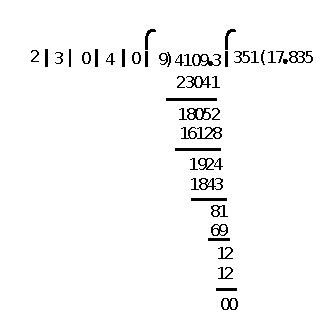
\includegraphics[scale=1.5]{5.eps}
\end{figure}

idaralilx BAjayxdalilxruva pUNARMkiyu $4109$ idanunx Bajakadalilxruva pUNARMki $230$ riMda BAgi\-salu BAgAkAradalilx eraDu pUNARMka sathxLagaLu uMTeMdu tiLiVtu. adaralilx koVrida aMsha sathxLagaLu $3$nunx sheVrisalu $5$ aMka  sAthxnagaLAdavu. Agalu $5$ aMka sathxLagaLanunx BajakadalilxTuTxkoMDu muMdakekx hecAcxda $9$nunx biTuTx biTiTxrutatxde. hAgeyeV A BajakAMkigaLiMda oMdu veVLe BAga hoVguvadakekx beVkAdaSuTx $5$ aMkigaLanunx iTuTx koMDu uLida $351$nunx biTuTx biTiTxrutatxde. A meVle, BAgisalAgi baMda vAyxLAyxMki $1$riMda $9$nunx guNisi, adara dashagi $1$ mAtarx tegadukoMDu, muMde guNisidadxralilx sheVrisi koMDu, baMda $23041$nunx kaLiyalAgi sheVSavu $18052$ uLadirutatxde. idanunx Bajakada $0$ sonenxyanunx biTuTx biTuTx, uLida $2304$riMda BAgisalAgi vAyxLAyxMkiyu $7$ baMtu. adariMda $0$ sonenxyanunx guNisidare, sonenxyeV Agutatxde. AdadxriMda dashagi bara\-lilalxveMdu tiLidu muMde guNisi kaLiyalAgi $1924$ uLiVtu. idanunx punaH Bajakadalilx $4$nunx biTuTx uLida $230$riMda meVlina karxmavAgi BAgisalu, vAyxLAyxMki $8$ baMtu. idariMda Bajakada $4$nunx guNisalu $32$, idakekx Aguva dashagiyu $3$, idanunx muMdina Bajakada guNakadalilx sheVrisikoMDu kaLiyalu $81$ uLiVtu. idanunx Bajakadalilxna $0$ sonenxyanunx biTuTx, uLida $23$riMda BAgi\-salu, vAyxLAyxMki $3$ baMtu. idariMda sonenxyanunx guNisalu dashagi baralilAlx. muMde $23$nunx guNisalAgi Ada $69$nunx kaLiyalAgi $12$ uLiVtu. idanunx Bajakada $3$nunx biTuTx uLida $2$riMda BAgisalu, vAyxLAyxMki $5$ baMtu. idariMda Bajakada $3$nunx guNisalu $15$, idakekx $2$ dashagi, AdadxriMda idanunx $5$riMda $2$nunx guNisi sheVrisalu $12$ Ayitu. idanunx kaLiyalu sheVSa uLiyalilalxvu Aga baMda BAga labadhxvu $17835$, idaralilx koVridaMthA $3$ aMsha sathxLagaLanunx biTuTx biMduvanunx mADirutatxde.\\

$2.5 \div .32$
\begin{figure}[H]
\centering
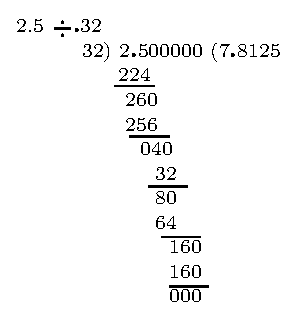
\includegraphics[scale=1.2]{3.eps}
\end{figure}

I leKaKxda BAjayxdalilx $6$ dashAMshagaLAgirutatxve, adaralilx Bajakadalilxruva $2$ dashAMsha sathxLagaLanunx kaLadare, uLi\-yuva $4$ dashAMsha sathxLagaLanunx labadhxdalilx biTuTx, biMduvanu mADirutatxde.

\begin{center}
{\bf \large 61neV aBayx udAharaNe.}
\end{center}

\begin{tabular}{>{$}c<{$}>{}l<{}>{}l<{}>{}l<{}>{}l<{}>{}l<{}}
(1) & $12.5 \div .5$ & (2) & $1.25 \div .54$ & (3) & $.125 \div .5$\\[10pt]
(4) & $12.5 \div .25$ & (5) & $164.65322 \div 5.132$\\[10pt]
(6) & $63.8976 \div 20.8$ & (7) & $359.23745 \div 67.21$\\[10pt]
(8) & $632648.66 \div 4.207$ & (9) & $555530199.62 \div 63.7054$\\[10pt]
(10) & $132.16 \div .0025$ & (11) & $.424 \div .000045$\\[10pt]
(12) & $.25 \div .000005$ & (13) & $9.065 \div .049$\\[10pt]
(14) & $576.\div .00000144$ & (15) & $125.\div .0000812$
\end{tabular}


